\documentclass{article}
\usepackage{tikz}
\usetikzlibrary{arrows.meta}
\usepackage{tkz-berge}

\begin{document}

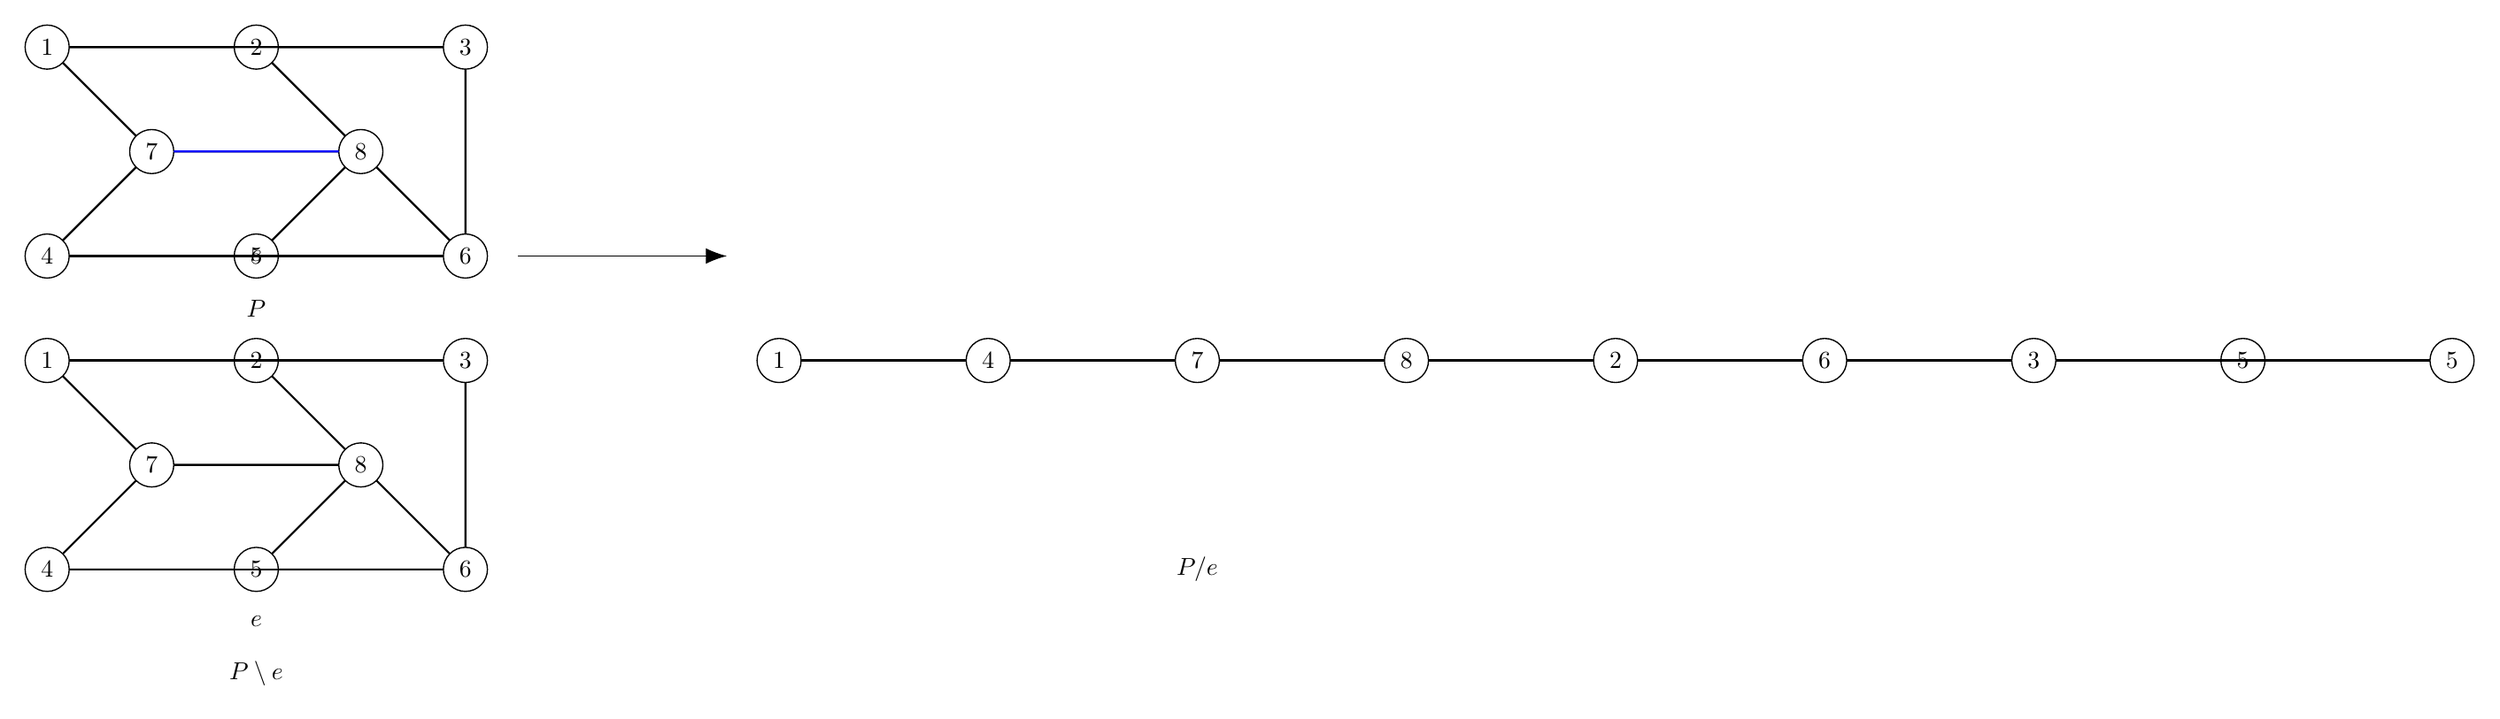
\begin{tikzpicture}[scale=1.5]
    % Define the nodes for the upper graph
    \Vertex[x=0,y=3]{1}
    \Vertex[x=2,y=3]{2}
    \Vertex[x=4,y=3]{3}
    \Vertex[x=0,y=1]{4}
    \Vertex[x=2,y=1]{5}
    \Vertex[x=4,y=1]{6}
    \Vertex[x=1,y=2]{7}
    \Vertex[x=3,y=2]{8}
    
    % Draw edges for the upper graph
    \Edges(1,2,3,1)
    \Edges(4,5,6,4)
    \Edges(1,7,4)
    \Edges(2,8,5)
    \Edges(3,6,8)
    \Edges(7,8)
    
    % Draw the edge e in blue
    \Edges[style={blue}](7,8)
    
    % Label the edge e
    \node at (2,1) {$e$};
    
    % Draw the label P
    \node at (2,0.5) {$P$};
    
    % Draw the arrow for the quotient map
    \draw[-{Latex[length=3mm]}] (4.5,1) -- (6.5,1);
    
    % Define the nodes for the lower graph
    \Vertex[x=0,y=0]{1}
    \Vertex[x=2,y=0]{2}
    \Vertex[x=4,y=0]{3}
    \Vertex[x=0,y=-2]{4}
    \Vertex[x=2,y=-2]{5}
    \Vertex[x=4,y=-2]{6}
    \Vertex[x=1,y=-1]{7}
    \Vertex[x=3,y=-1]{8}
    
    % Draw edges for the lower graph
    \Edges(1,2,3,1)
    \Edges(4,5,6,4)
    \Edges(1,7,4)
    \Edges(2,8,5)
    \Edges(3,6,8)
    \Edges(7,8)
    
    % Draw the edge e in black
    \Edges(7,8)
    
    % Label the edge e
    \node at (2,-2.5) {$e$};
    
    % Draw the label P \setminus e
    \node at (2,-3) {$P \setminus e$};
    
    % Define the nodes for the quotient graph
    \Vertex[x=7,y=0]{1}
    \Vertex[x=9,y=0]{4}
    \Vertex[x=11,y=0]{7}
    \Vertex[x=13,y=0]{8}
    \Vertex[x=15,y=0]{2}
    \Vertex[x=17,y=0]{6}
    \Vertex[x=19,y=0]{3}
    \Vertex[x=21,y=0]{5}
    \Vertex[x=23,y=0]{5}
    
    % Draw edges for the quotient graph
    \Edges(1,4,7,8,2,6,3,5)
    
    % Label the quotient graph
    \node at (11,-2) {$P/e$};
\end{tikzpicture}

\end{document}